\chapter{Durchführung}
\label{cha:Durchführung}

Die Messapparatur zur Oberflächenuntersuchungen mittels Röntgenreflektometrie ist in Abbildung \ref{fig:Aufbau} dargestellt. In dieser Abbildung befindet sich die Röntgenröhre bei 
Position (a). Gegenüber befindet sich der Detektor an Position (c). Sowohl der Detektor als auch die Röntgenröhre sind drehbar durch die Vorrichtung mittig im Hintergrund. 
Die zu vermessende Probe befindet sich an Position (b). Die Probe kann durch eine Stage in alle Richtungen verfahren werden, welche sich an Position (d) befindet. Der ganze Aufbau 
befindet sich hinter Sicherheitsglas, welches verhindert, dass ein Mensch in den Strahlengang kommen kann. Die Apparatur wird über einen Computer gesteuert.  

\begin{figure}
    \centering
    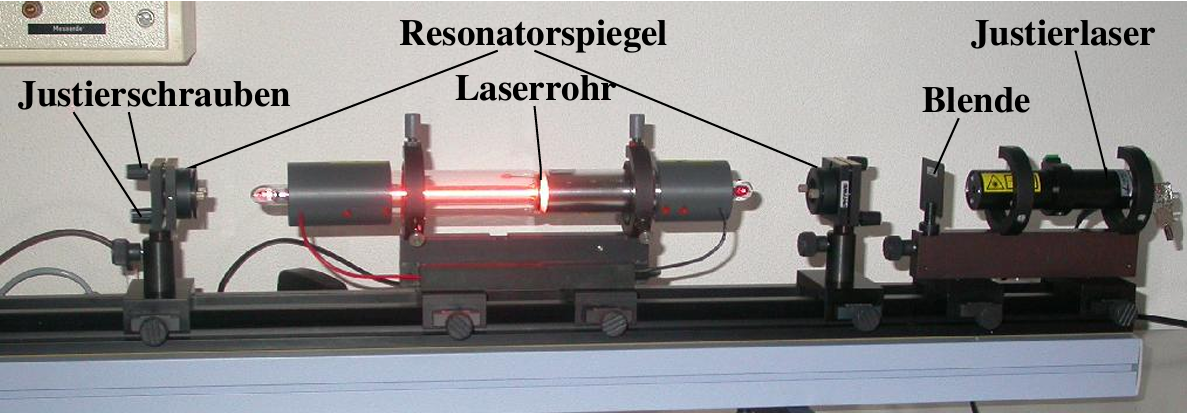
\includegraphics[width=0.9\textwidth]{content/Bilder/Aufbau.pdf}
    \caption{Bild des verwendeten Diffraktometers. \textbf{(a)} Röntgenröhre, \textbf{(b)} Probe, \textbf{(c)} Detektor, \textbf{(d)} xyz-Messtisch.}
    \label{fig:Aufbau}
\end{figure}

Bevor mittels Röntgenreflektometrie die Dichte, Rauigkeit und die Dicke eines Polysterolfilms auf einem Siliziumwafer gemessen werden kann, muss die Messapparatur justiert werden. 
Dafür werde eine Reihe an Scans durchgeführt um die Probe vernünftig zu positionieren und Störfaktoren zu berechnen. Zuerst muss ein Detektorscan durchgeführt werden. Für diesen 
wird die Probe vollständig aus dem Strahlengang gefahren. Dann wird der Detektor relativ zur Röntgenröhre gedreht und dabei die Intensität vermessen. Dies ist notwendig, damit das 
Signal im Detektor möglichst hoch ist. Daher speichert der Detektor nach dem Scan die Position mit der höchsten Intensität als standardwert ab. 

Dann wird ein Z-Scan durchgeführt. Bei diesem wird die Probe langsam in den Strahlengang gefahren und es wird erneut die Intensität gemessen. Dieser Scan ist notwending um die 
z-Position der Probe so zu wählen, dass diese soeben beschienen wird.

Darauf hin wird ein X-Scan durchgeführt. Dieser gewährleistet, dass die Probe in der Korrekten x-Position liegt und eine maximale Beleuchtung verwendet wird. 

Weiter wird ein Rocking-Scan für den Winkel $2\Theta = \qty{0}{\degree}$ durchgeführt. Dieser passt nun die y-Position der Probe an in dem der Winkel auf das Maximum geeicht wird. 

Für eine qualitative Justage ist es notwendig noch einen weiteren Z-Scan, Rocking-Scan mit $2\Theta = \qty{0.3}{\degree}$, ein Z-Scan und einen letzten Rocking-Scan mit 
$2\Theta = \qty{0.5}{\degree}$ durchzuführen. Die Messbereiche der verwendeten Scans sind in Tabelle \ref{tab:Messbereiche} zusammengefasst.

\begin{table}
    \centering
    \caption{Darstellung der zu verwendenden Messbereiche der einzelnen Justagescans.}
    \label{tab:Messbereiche}
    \begin{tabular}{l c}
      \toprule
      {Typ} & {Messbereich} \\
      \midrule
      {Detektorscan}                & {$\numrange{-0,5}{0,5}$}  \\
      {Z-Scan}                      & {$\numrange{-1}{1}$}      \\
      {X-Scan}                      & {$\numrange{-20}{20}$}    \\
      {Rockingscan $2\theta=0$}     & {$\numrange{-1}{1}$}      \\
      {Z-Scan}                      & {$\numrange{-0,5}{0,5}$}  \\
      {Rockingscan $2\theta=0,3$}   & {$\numrange{0}{0,3}$}     \\
      {Z-Scan}                      & {$\numrange{-0,5}{0,5}$}  \\
      {Rockingscan $2\theta=0,3$}   & {$\numrange{0,2}{0,5}$}   \\
      \bottomrule
    \end{tabular}
\end{table}

Nach eine erfolgreichen Justage kann die Reflektivitätsmessung begonnen werden. Der Messbereich lautet $\qty{0}{\degree}$ bis $\qty{2.5}{\degree}$. Für eine ausreichende 
Datenmenge sollte eine Schrittweite von $\qty{0.005}{\degree}$ mit jeweiliger Messdauer von $\qty{5}{\second}$ gewählt werden. Um Streueinflüsse zu verhindern muss außerdem ein 
Diffuse-Scan durchgeführt werden. Dafür werden die Einstellungen bei behalten, allerdings wird der Detektor um $\qty{0.1}{\degree}$ verfahren, damit dieser nur gestreute Signale 
misst. Mit dem Diffuse-Scan wird in der Auswertung die Reflektivität korrigert.